\begin{savequote}[8cm]
\textlatin{Neque porro quisquam est qui dolorem ipsum quia dolor sit amet, consectetur, adipisci velit...}

There is no one who loves pain itself, who seeks after it and wants to have it, simply because it is pain...
  \qauthor{--- Cicero's \textit{de Finibus Bonorum et Malorum}}
\end{savequote}

\chapter{\label{ch:1-intro}Introduction} 

\minitoc

\section{Motivation}

Intense star formation in galaxies as well as active galactic nuclei can drive the ejection of gas in different phaces (neutral, ionized, molecular) out of a galaxy.
The ejected gas, can reach up to hundreds to kiloparsec scales, becoming large--scale galactic outflows drived by SF-process, AGN activity or both.

Despite its plenity identification at low and high redshift (tipically constrained its detection between $0<z<2$), its main physical mechanism(s) that produces
and regulates its production is(are) still unclear. The most common mechanism to detect them is trough emission and absorption lines (molecular, optical, UV, NIR, soft Xray). 

The wind leaves signatues in the spectrum as broad or assimetric profiles, indicative of the precense of distint kinematic components as result of the propagion of the wind.
As more intense the wind energy source, higher the velocity. Therefore, a disturbed kinematic in the galaxy velocity field, is a condition to reveal the precense of an outflow (both AGN or SF driven), 
although this is not definitive. 
 
Given the large amount of energy  realezed ($\sim 10^{xx}$ erg s-1), and posterior inject back to the host galaxy, its
consequences might change the subsequent evolution of the host galaxy itself. 

The main energy sources that produce galactic scale outflows are: (i) Supernovae (SNe) explosions. Intense star formation rates as those present in starburst galaxies are prone to
develop large scale outflows. At the end of its life, massive stars (10 M$_{\odot}$) end up as SNe, the relative short live of these stars and its inmediate explosion as SNe
delivers amounts of energy to the ISM. The joint effect of multiple SN explosions drives as a expanding shell is now well uderstood (Heckman 1990). From this, it is not surprising that
the total energy of SNs is directly related with the globlal SFR of a galaxy. 


(ii) Nuclear activity. The accretion of material into super massive black holes (SMBH) in the center of galaxies can lead to the production of higly energetic outflows (AGN-driven), tipically preceded
by a radio jet. The more luminous the AGN is, major its velocity, reaching in the most luminous cases up to $~10^3$ \kms. 

Commonly the study of outflows has been performed over galaxy samples where its precesen is ubiquitous. This is, in galaxies with high star formation rates, in the 
so called ultra luminous infrared galaxies (ULIRGs), or in the most luminous AGNs, such as QSO. Although all these studies has contributed to expand our knoledge to the outflows phenomena.

All these studies have consolidated our current knowledge about the outflows, where to find them and how estimate its main physical properties,as well as the
limitations. Nowadays with the advent of large galaxy surveys it is possible to perform unbiased studies. One of the major questions that attend to answer in this thesis is
on how frequent they are, and why they seem to be  not ubiquitous in all galaxies. 
 

\section{Integral Field Spectroscopy}
In the late 90s and early 2000s, a new observation technique came to light to overcome the classical long slit spectroscopy. The
integral field spectroscopy (IFS) technique produces simultaneously multiple spatially resolved spectra over a two dimensional field \cite{bookIFS}. This technique
bringing back the study of extended objects, instead the one sigle fiber, or long slit spectroscopy. The IFS technique
provides a 3 dimensional vission of a galaxy, two dimensions $(x,y)$ corresponds to the spatiall  information (R.A.,Dec), and the $z$ axis corresponds to the wavelength axis.
How the information is recorded depends on the type of integral field unit (IFU). The most common are represented in Fig. \ref{fig:ifs}. 
The final reduction process results in a data cube, where each of its spatial elements (spaxels) records the spectroscopic information of a small portion of a galaxy. The gread advantage of this
technique is the possibility of study the individual structural components of galaxyes (such as bars, disk, bulge, spiral arms, \hii~regions etc.)

The large programs to study galaxies using the IFS technique started with the SAURON project \cite{bacon01}. SAURON was optimized to study the stellar kinematics of nearby early-type galaxies.
Followed SAURON, the SAMI Galaxy Survey \cite{samiOLD} came to light with more than $\sim 3400$ low redshift galaxies ($z<0.12$). 

The larger program in observed galaxies is the MaNGA survey \cite{mangaOLD}, aiming to observe $\sim 10000$ galaxies from the Local Universe. The CALIFA survey \cite{sanchez12a} is the last IFS galaxy
survey delivering $~800$ galaxies of the Local Universe. 

Many MUSE IFS projects has been proposed to study with high spatial resoluion the physical properties of low and high redshift galaxies. Although there is not yet a proper MUSE galaxy survey,
the AMUSING++ compilation has collected the major number of galaxies observed with MUSE so far. 

Table \ref{tab:IFS_properties} sumarizes the main properties of the main IFS galaxy surveys.

\begin{sidewaystable} 
\begin{tabular}{lllrlll}
\toprule
 Survey    & redshift      & R         &   N\_gal & FWHM (arcsec)   & FoV (arcsec)   & lambda\_range (Angs)   \\
\midrule
 SAMI      & 0.004\ensuremath{<}z\ensuremath{<}0.092 & 1700,4500 &    1559 & 2.16            & 15x15          & 3700--7300            \\
 MaNGA     & 0.025\ensuremath{<}z\ensuremath{<}0.15  & 1400-2600 &   10000 & 2.54,2.48       & 7-32           & 4000--9000            \\
 CALIFA    & 0.005\ensuremath{<}z\ensuremath{<}0.03  & 850,1650  &     667 & 2.5             & 78x73          & 3745--7500            \\
 AMUSING++ & 0.001\ensuremath{<}z\ensuremath{<}0.1   & 3000      &     700 & seeing limited  & 60x60          & 4800--9300            \\
\bottomrule
\end{tabular}
\label{tab:IFS_properties}
\caption{Main IFS galaxy surveys}
\end{sidewaystable} 


\begin{figure}
\centering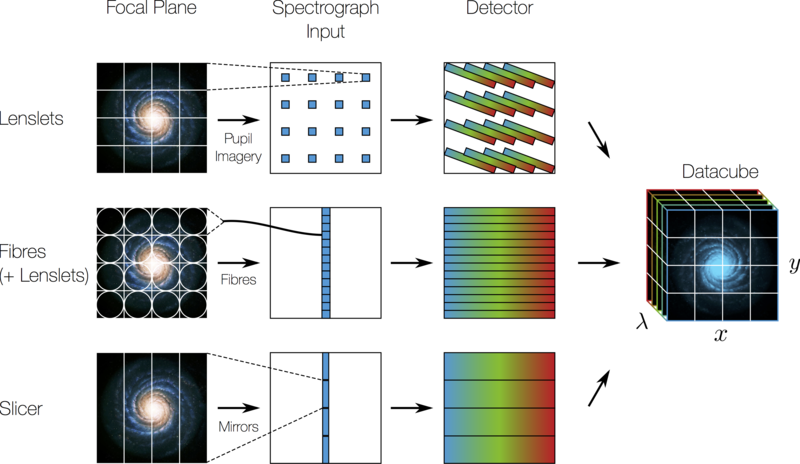
\includegraphics[width=0.7\textwidth]{figures/ifs.png} 
\caption[]{Diffeerent types of IFU. }
\label{fig:ifs}
\end{figure}


\section{Data}
The current work is based on data from extracted from the CALIFA survey \url{https://califa.caha.es} and MUSE data \url{http://ifs.astroscu.unam.mx/AMUSING++}.

\subsection{CALIFA}
The CALIFA project has been one of the most successful IFS galaxy surveys, mostly because of its well-designed sample.
CALIFA is a diameter selection sample, covering up to 2 effective radius (R$_e$) in the vast majority of the galaxies. 
The diameter selection condition allowed to perform volume corrections over the sample within
the redshift range of the galaxies. This great adventage has allowed to estimate statistical properties of the sample, and therefore of the Local Universe. 

The vast coverage of the blue and red part of the optical spectrum allows recovering the information of the stellar component trough the appropriate SSP fitting analysis techniques. Moreover, the most prominent emission lines in the optical spectrum are totally sampled.

Given its large FoV, the CALIFA galaxies can be studied spatially resolved (spaxel-by-spaxel), globally (integrated) or radially. Therefore, the way in which galaxies are studied 
has changed dramatically with the adevent of the most modern IFS techiques, particulary with the CALIFA survey has opened a branche towards the 3 dimensional study of galaxies.

\subsection{MUSE}

Installed at the  Very Large Telescope in the southern hemisphere, the Multi Unit Spectroscopic Explorer (MUSE) is the most modern instrument for obtaining IFS data in the optical. MUSE
provides a high spatial resolution limited by the local seeing, and a moderated spectral resolution that depends on the wavelength. For the lowest redshift galaxies, MUSE can 
achive spatial resolutions of the order of $\sim 100$ pc (cite TIMER,MAD), pushing to the limit the established global scaling relations of galaxies, 
at unprecedent resolutions. 

Many extragalactic projects has been proposed to study the physical properties of galaxies at different scales.

The major disadvanatge of the current MUSE, is the lack of the blue part of the spectrum. 
Important absorptions lines in the blue part of the spectrum can help to break the well known age-metallicity degeneracy. 
A direct consequence of this degeneracy is the unreliability in the SSP analysis on the MUSE data cubes. 
Nevertheless, this degeneray do not affect the extraction of ionized gas properties.

Keeping in mind this caveat, many extragalactic projects has been proposed to study the physical
properties (particularly on the ionized gas) of galaxies at different scales. 

In this thesis, data from the public ESO archive has been used, in combination with data from other major MUSE programs, as it will be described in further sections.

%In general older stellar populations are redder, like metal rich ones, while younger and metal poor ones are bluer (Worthey 1994). This in troduces a degeneracy in the derivation of both parameters, as discussed by previous authors

\section{Data Analysis}

The spectra observed in a region of galaxy is the result of the contribution of all ionizing and continuum sources in that region. Particularly, at the redshift range of the
previous IFS galaxy surveys, the initial mass function (IMF) is not sampled at any of the previously cited spatial resolutions. Therefore, it is assumed that
in each spatiall element in a galaxy, the observed continuum spectrum is the combination of the sum of some thousands of stars, giving the shape of the continuum spectra in each spaxel.  

In order to recover the ionized and stellar content of galaxies, we perform a simple stellar population analys (SSP) analysis to each spectra of the datacubes.
To achive this, we use the {\sc Pipe3d} \cite{Pipe3D_I}, a fitting routine adapted to analyse IFS  data using the package {\sc FIT3d} \cite{Pipe3D_II}. A wide description
of how {\sc Pipe3d} works is described in  \cite{Pipe3D_I}. In general terms, this routine performs a decomposition of the original spectrum into SSP, 
prior to a coadding of adjacent spectra process in order to increase the \SN~of the continuum. This results in a segmented map of the galaxy in question. 
Over each segmented bin, also known as tessela, a SSP fitting is perfomed over the coaddes spectra. 
SSP templates of different ages and metallicities are used to perform this analysis. The fit is then monitored with a chi-squared minimization process. 
The final SSP model, contains information of the mean age, stellar mass and stellar metallicities. This is choosen as representative SSP model of the tessela. After that
an dezonification process is performed, to recover the . An example of this fitting procedure is sumarized in Fig. \ref{fig:ssp_fitting}. 

Once obtained the best SSP model, this is subtracted to the original spectra to obtain a spectrum free of stellar-continuum, this is, a gas
spectra dominated by pure emission lines (plus some residual noise). After this, the emission lines are fitted trough a moment analysis procedure to recover the flux, 
velocity and velocity dispersion with its corresponding errors for each analized emission line.

The previous proccedure applied to a entire datacube, produces a set of 2D maps of the stellar and ionized components. {\sc Pipe3d} packs the results of 
the analysis in datacubes, separated in the stellar and ionized gas information. These products are named dataproducts. 


\begin{figure*}
\centering
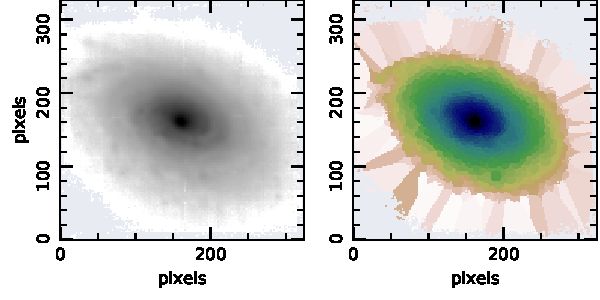
\includegraphics[width= \textwidth]{figures/tessela.pdf} 
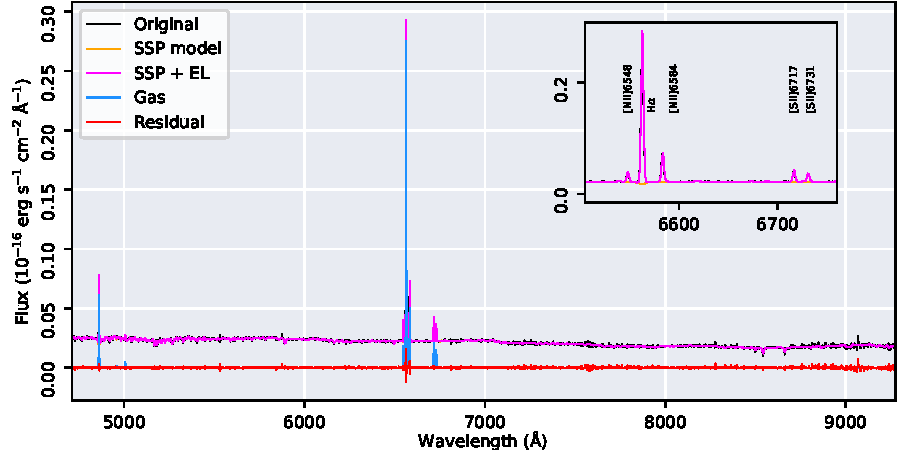
\includegraphics[width= \textwidth]{figures/ssp_fit_muse.pdf} 
\caption[]{Example of the SSP analysis applied to an IFS cube. In this example only a single spectrum of a tessela is analyzed. 
{\it Top left:} V--band continuum image extracted from the datacube. {\it Top right:} Tesselation map. 
{\it Bottom panel:} The {\sc Pipe3d} routine models the obseved spectra (black) with a combination of different SSP, the best model (orange) is
considered as the best   }
\label{fig:ssp_fitting}
\end{figure*}










